\chapter{Binary Classiciation at the Top}\label{chap: framework}

In the previous chapter, we introduced the general formulation~\eqref{eq: Binary classification counts} and fundamental evaluation matrices for the binary classification problems. Furthermore, in Section~\ref{sec: related problems}, we introduced three problems closely related to binary classification but focused on specific performance criteria. Namely: \emph{Accuracy at the top} problem, \emph{Ranking problems}, and the problem of \emph{Hypothesis testing}. Even though these problems are usually considered separately, they have one crucial thing in common. All three problems aim to minimize the number of misclassified samples below (or above) a certain threshold. In the rest of the chapter, we focus on this common property. We show that all these problems fall into the following unified framework for binary classification at the top
\begin{mini}{\bm{w}}{
  \lambda_1 \cdot \fp(\bm{s}, t) + \lambda_2 \cdot \fn(\bm{s}, t)
}{\label{eq: aatp counts}}{}
  \addConstraint{s_i}{= f(\bm{x}_i; \bm{w}), \quad}{i \in \I}
  \addConstraint{t}{= G\Brac{\bm{s}, \bm{y}},}
\end{mini}
where function~$G \colon \R^n \times \{0, 1\}^n \to \R$ takes the scores and labels of all samples and computes the decision threshold. The concrete form of the function~$G$ that defines the decision threshold depends on the used problem. As we show later in the chapter, all problems mentioned above differ only in the definition of the function~$G.$  Note the important distinction from the standard binary classification~\eqref{eq: Binary classification counts}: the decision threshold is no longer fixed (as in the case of neural networks) or trained independently (as in SVM) but is a function of scores of all samples. Therefore, the minimization in problem~\eqref{eq: aatp counts} is performed only concerning the one variable~$\bm{w}.$

\section{Surrogate formulation}\label{sec: surrogate formulation}

The objective function of problem~\eqref{eq: aatp counts} is a weighted sum of false-positive and false-negative counts. Since these counts are discontinuous due to the presence of the Iverson function (see~\eqref{eq: confusion counts}), the whole objective function is discontinuous too. Therefore, problem~\eqref{eq: aatp counts} is difficult to solve. One way how to simplify the problem is to derive its continuous approximation. Since the only discontinuous part of the objective function is the Iverson function, the usual approach is to employ a surrogate function to replace it~\cite{li2014top, grill2016learning}.

\begin{notation}[Surrogate function]\label{not: surrogates}
  In the text below, the symbol~$l$ denotes any convex non-negative non-decreasing function with~$l(0) = 1$. As examples of such function we can mention the hinge loss function or the quadratic hinge loss functions defined as follows
  \begin{align*}
    l_{\text{hinge}}(s) & = \max\Brac[c]{0, 1 + s}, &
    l_{\text{quadratic}}(s) & = \Brac{\max\Brac[c]{0, 1 + s}}^2.
  \end{align*}
  Moreover, parameter~$\vartheta > 0$ is used to scale inputs to any surrogate function.
\end{notation}

Notation~\ref{not: surrogates} summarizes all assumptions that a proper surrogate function must fulfill and introduces the two most often used surrogate functions: hinge and quadratic hinge loss functions. Moreover, Figure~\ref{fig: surrogates} compares these two surrogate functions with the Iverson function. It is clear that the surrogate function always provides  an upper approximation of the Iverson function. In other words, if a surrogate function~$l$ satisfies assumptions from Notation~\ref{not: surrogates}, then~$l(s) \geq \Iverson{s \geq 0}$ holds for any~$s \in \R.$ Besides that, Figure~\ref{fig: surrogates} shows how the scaling parameter~$\vartheta$ affects the approximation quality of the surrogate function. If the scaling parameter is greater than 1, the surrogate function approximates the Iverson function better on interval~$(-\infty, 0)$. In the opposite case, the approximation is better on interval~$(0, \infty)$. The usual choice of scaling parameter is~$\vartheta = 1,$ and we used this choice for all surrogate functions used in the objective functions. However, we also use surrogate functions for approximation of the decision threshold. In such a case, the scaling parameter plays a crucial role for some theoretical guaranties, as shown in upcoming chapters.

\begin{figure}[t]
  \centering
  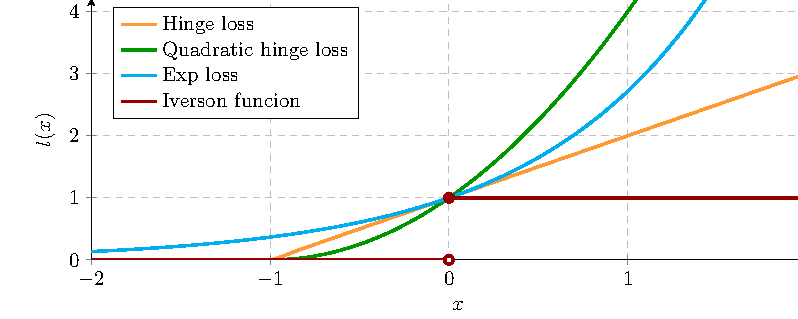
\includegraphics[width = \linewidth]{images/surrogates.pdf}
  \caption{Comparison of the approximation quality of the Iverson function using different surrogate functions and scaling parameters.}
  \label{fig: surrogates}
\end{figure}

With a properly defined surrogate function, we can define the surrogate approximation of the objective function of problem~\eqref{eq: aatp counts}. To follow the notation from the previous chapter, we first replace the Iverson function in~\eqref{eq: aatp counts}. Using any surrogate function~$l$ that satisfies assumptions from Notation~\ref{not: surrogates}, the true counts~\eqref{eq: aatp counts} may be approximated by their surrogate counterparts defined by
\begin{equation}\label{eq: confusion counts surrogate}
  \begin{aligned}
    \tps(\bm{s}, t) & = \sum_{i \in \Ipos}l(s_i - t), & \qquad
    \fns(\bm{s}, t) & = \sum_{i \in \Ipos}l(t - s_i), \\
    \tns(\bm{s}, t) & = \sum_{i \in \Ineg}l(t - s_i), &
    \fps(\bm{s}, t) & = \sum_{i \in \Ineg}l(s_i - t).
  \end{aligned}
\end{equation}
Since the surrogate function provides upper approximation of the Iverson function, the surrogate counts~\eqref{eq: confusion counts surrogate} provide upper approximations of the true counts~\eqref{eq: confusion counts}. By replacing the true counts in the objective function of~\eqref{eq: aatp counts} with their surrogate counterparts and adding a regularization for better numerical stability, we get
\begin{mini}{\bm{w}}{
  \frac{1}{2} \norm{\bm{w}}^2 + \lambda_1 \cdot \fps(\bm{s}, t) + \lambda_2 \cdot \fns(\bm{s}, t)
  }{\label{eq: aatp surrogate}}{}
  \addConstraint{s_i}{= f(\bm{x}_i; \bm{w}), \quad i \in \I}
  \addConstraint{t}{= G\Brac{\bm{s}, \bm{y}}.}
\end{mini}
The resulting objective function is continuous, and therefore the problem is easier to solve than the original problem~\eqref{eq: aatp counts}. No additional theoretical properties can be derived without knowing the concrete form of model~$f$ and function~$G.$ Therefore, the rest of the chapter is dedicated to problems that fall into the general framework~\eqref{eq: aatp surrogate} and concrete form of~$G$ for such problems. More precisely, we focus on the three problems introduced in Section~\ref{sec: related problems} and show how to rewrite them to our general formulation~\eqref{eq: aatp surrogate}. Most of these problems are defined originally only for the linear model since this choice allows to derive nice theoretical properties and efficient solving algorithms. However, this chapter focuses on the problem formulation itself rather than on how to solve it. Therefore for all problems, we derive their version with general model~$f.$ The discussion of the theoretical properties for specific forms of~$f$ is provided in Chapter~\ref{chap: linear},~\ref{chap: dual}, and~\ref{chap: deep}.

\begin{notation}[Classification scores]\label{not: scores}
  In Notation~\ref{not: classifier}, we defined vector~$\bm{s} \in \R^n$ of scores of all samples with components defined for any~$i \in \I$ as
  \begin{equation*}
    s_i = f(\bm{x}_i; \bm{w}), \quad i \in \I,
  \end{equation*}
  where~$f \colon \R^d \to \R$ represents an arbitrary model. To simplify the upcoming sections, we define a sorted version of vector~$\bm{s}$ with decreasing components and denote it as~$\bm{s}_{[\cdot]}.$ It means that components of~$\bm{s}_{[\cdot]}$ fulfill
  \begin{equation*}
    s_{[1]}   \geq s_{[2]} \geq \dots \geq s_{[n - 1]} \geq s_{[n]}.
  \end{equation*}
  Moreover, we denote negative samples as~$\bm{x}^-$ and positive samples as~$\bm{x}^+.$ Finally, we define vectors~$\bm{s}^- \in \R^{\nneg},$ $\bm{s}^+ \in \R^{\npos}$ of scores of all positive and negative samples with components defined as
  \begin{equation*}
    \begin{aligned}
      s^-_j & = f(\bm{x}^-_j; \bm{w}), \quad j = 1, \; 2, \ldots, \; \nneg, \\
      s^+_i & = f(\bm{x}^+_i; \bm{w}), \quad i = 1, \; 2, \ldots, \; \npos,
    \end{aligned}
  \end{equation*}
  and their sorted versions~$\bm{s}^-_{[\cdot]}$, $\bm{s}^+_{[\cdot]}$ with decreasing components.
\end{notation}

\section{Ranking problems}\label{sec: ranking}

The first category of problems from Section~\ref{sec: related problems} is a category of ranking problems. The general goal of problems from this category is to rank positive (relevant) samples higher than negative ones. That can be achieved in many different ways, but we focus only on the problems that concentrate on the high-ranked negative samples and try to push as many positive samples as possible above them. The simplest case is when the goal is to maximize the number of positive samples above the worst negative. Since the worst negative sample is the negative sample with the highest classification score, the decision threshold for such a case is the highest score corresponding to the negative sample. Then the aim is to maximize the number of true-positive samples above this threshold or, equivalently, minimize the number of false-negative negative below it, which may be written as
\begin{mini}{\bm{w}}{
  \frac{1}{\npos} \fn(\bm{s}, t)
  }{\label{eq: toppush}}{}
  \addConstraint{s_i}{= f(\bm{x}_i; \bm{w}), \quad i \in \I}
  \addConstraint{t}{= s_{[1]}^-}
\end{mini}
Note that the decision threshold~$t$ in the previous formulation is a function of classification scores. Therefore, the formulation is just a special case of the general formulation~\eqref{eq: aatp counts} for $\lambda_1 = 0$ and~$\lambda_2 = \nicefrac{1}{\npos}$. The authors in~\cite{li2014top} proposed an efficient method to solve formulation~\eqref{eq: toppush} and called it \TopPush. They replaced the true counts in the objective function of~\eqref{eq: toppush} with its surrogate counterpart in the same way as we did in Section~\ref{sec: surrogate formulation}. The resulting formulation has the following form
\begin{mini}{\bm{w}}{
  \frac{1}{2} \norm{\bm{w}}^2 + \frac{1}{\npos} \fns(\bm{s}, t)
  }{\label{eq: toppush surrogate}}{}
  \addConstraint{s_i}{= f(\bm{x}_i; \bm{w}), \quad i \in \I}
  \addConstraint{t}{= s_{[1]}^-,}
\end{mini}
which again falls into our framework~\eqref{eq: aatp surrogate}. To stress the origin of this formulation, we denote it as \TopPush. Unfortunately, \TopPush formulation can be very sensitive to outliers, especially when the linear model is used, as shown in~\ref{sec: stability}. To robustify the formulation, we follow the idea presented in~\cite{lapin2015top} and replace the highest negative score by the mean of~$K$ highest negative scores. The resulting formulation is as follows
\begin{mini}{\bm{w}}{
  \frac{1}{2} \norm{\bm{w}}^2 + \frac{1}{\npos} \fns(\bm{s}, t)
  }{\label{eq: toppushK surrogate}}{}
  \addConstraint{s_i}{= f(\bm{x}_i; \bm{w}), \quad i \in \I}
  \addConstraint{t}{= \sum_{i = 1}^{K} s_{[i]}^-},
\end{mini}
To emphasize the similarity with the \TopPush, we call this formulation \TopPushK. It is also possible to use the value of $K$-th highest negative score as the threshold. Such a choice may be advantageous in some cases, and we will discuss it in Chapter~\ref{chap: deep}. For now, we will stick to the formulation that uses the mean since it will allow us to derive some crucial theoretical properties, as shown in Section~\ref{sec: convexity}. 

\section{Accuracy at the Top}\label{sec: aatp}

The second problem from Section~\ref{sec: related problems} is the problem of Accuracy at the Top~\cite{boyd2012accuracy}. This problem aims to find an ordering of samples so that samples whose scores are among the top $\tau$-quantile are as relevant as possible. The top~$\tau$-quantile of all scores is defined by
\begin{equation}\label{eq: aatp quantile} 
  t_1(\bm{s})
    = \max \Set{t}{\frac{1}{n} \sum_{i \in \I} \Iverson{s_i \geq t} \geq \tau}.
\end{equation}
All relevant samples should be ranked above the quantile~$t_1$ and all irrelevant samples below the quantile~$t_1$ in an ideal case. Thus, the main difference to the ranking problems is that the problem of Accuracy at the Top considers both classification errors and does not focus only on false-negative samples. The original formulation~\cite{boyd2012accuracy} considers a balanced dataset with the same number of positive and negative samples. Paper~\cite{grill2016learning} reformulated the problem for the unbalanced dataset and derived the following formulation
\begin{mini}{\bm{w}}{
  \frac{1}{\nneg} \fp(\bm{s}, t) + \frac{1}{\npos} \fn(\bm{s}, t)
  }{\label{eq: aatp}}{}
  \addConstraint{s_i}{= f(\bm{x}_i; \bm{w}), \quad i \in \I}
  \addConstraint{t}{= \max \Set{t}{\frac{1}{n} \sum_{i \in \I} \Iverson{s_i \geq t} \geq \tau}.}
\end{mini}
This formulation already falls into our framework~\eqref{eq: aatp counts} for~$\lambda_1 = \nicefrac{1}{\nneg}$ and~$\lambda_2 = \nicefrac{1}{\npos}$. Moreover, the authors of~\cite{boyd2012accuracy, grill2016learning} used the same surrogate trick to get rid of the discontinuous objective function, as we used in Section~\ref{sec: surrogate formulation}. Thus, by replacing replaces false-positive and false-negative counts in the objective function with their surrogate counterparts we get
\begin{mini}{\bm{w}}{
  \frac{1}{2} \norm{\bm{w}}^2 + \frac{1}{\nneg}\fps(\bm{s}, t) + \frac{1}{\npos} \fns(\bm{s}, t)
  }{\label{eq: grill}}{}
  \addConstraint{s_i}{= f(\bm{x}_i; \bm{w}), \quad i \in \I}
  \addConstraint{t}{= \max \Set{t}{\frac{1}{n} \sum_{i \in \I} \Iverson{s_i \geq t} \geq \tau}.}{~}
\end{mini}
This formulation falls into our framework~\eqref{eq: aatp surrogate} for~$\lambda_1 = \nicefrac{1}{\nneg}$ and~$\lambda_2 = \nicefrac{1}{\npos}$. Even though the original formulation is presented in~\cite{boyd2012accuracy}, we denote the previous formulation as \Grill based on the name of the first author of~\cite{grill2016learning}. There are two reasons for that. The first one is that we used an unbalanced dataset as in~\cite{grill2016learning}. The second one is that we use an algorithm proposed in~\cite{grill2016learning} for numerical experiments since the one from~\cite{boyd2012accuracy} is suitable only for a small dataset.

The \Grill formulation~\eqref{eq: grill} is still challenging to solve due to the form of the decision threshold~\eqref{eq: aatp quantile}. The authors of~\cite{boyd2012accuracy} removed the necessity to handle the difficult quantile constraint by setting quantile as one of the samples and solving~$\nall$ independent problems. However, such an approach is infeasible for a large number of samples. The authors of~\eqref{eq: grill} proposed the projected gradient descent method, where after each gradient step, the quantile is recomputed. This approach is suitable for large data but lacks theoretical guarantees. In the following text, we propose two approximations of the true quantile~\eqref{eq: aatp quantile} that can be used to simplify formulation~\eqref{eq: grill}. The first one is a simple approximation by the mean of~$n\tau$ highest scores
\begin{equation}\label{eq: aatp quantile mean} 
  t_2(\bm{s}) = \frac{1}{n\tau} \sum_{i=1}^{n\tau} s_{[i]}.
\end{equation}
where for simplicity we assume, that~$n\tau$ is an integer. The main purpose of~\eqref{eq: aatp quantile mean} is to provide a convex approximation of the non-convex quantile~\eqref{eq: aatp quantile}. In fact, it is known is that it is the tightest convex approximation of~\eqref{eq: aatp quantile}. Putting~\eqref{eq: aatp quantile mean} into the constraint results in the following problem, which we call \TopMeanK
\begin{mini}{\bm{w}}{
  \frac{1}{2} \norm{\bm{w}}^2 + \frac{1}{\npos} \fns(\bm{s}, t)
  }{\label{eq: topmeank}}{}
  \addConstraint{s_i}{= f(\bm{x}_i; \bm{w}), \quad i \in \I}
  \addConstraint{t}{= \frac{1}{K} \sum_{i=1}^{K} s_{[i]},}
\end{mini}
where~$K = n\tau.$ Besides changing the form of the decision threshold, we also simplified the objective function. This change allows preserving the convexity of the formulation for the linear model as shown in Section~\ref{sec: convexity}. The resulting formulation is very similar to the \TopPushK formulation from the previous section. The only difference is that the threshold for \TopMeanK is computed from scores of all samples and not only from the negative ones.

The second option how to approximate the true quantile is to use surrogate counterparts to replace true counts in~\eqref{eq: aatp quantile} and solve the following equality
\begin{equation}\label{eq: aatp quantile surrogate}
  t_3(\bm{s}) \quad \text{solves} \quad \frac{1}{n}\sum_{i \in \I} l\Brac{\vartheta(s_i - t)} = \tau, 
\end{equation}
where~$\vartheta > 0$ is scaling parameter. Since this threshold uses the surrogate approximation, we denote it as surrogate top $\tau$-quantile. We get the following formulation by replacing the true quantile in the constrain and simplifying the objective function
\begin{mini}{\bm{w}}{
  \frac{1}{2} \norm{\bm{w}}^2 + \frac{1}{\npos} \fns(\bm{s}, t)
  }{\label{eq: patmat}}{}
  \addConstraint{s_i}{= f(\bm{x}_i; \bm{w}), \quad i \in \I}
  \addConstraint{t}{\quad \text{solves} \quad \frac{1}{n}\sum_{i \in \I} l\Brac{\vartheta(s_i - t)} = \tau.}
\end{mini}
This formulation also used only false negatives in the objective to preserve the convexity for the linear model. In such a case, the formulation is easily solvable due to the convexity and requires almost no tuning. Together with the fact that formulation~\eqref{eq: patmat} provides a good approximation to the Accuracy at the Top problem, we named it \PatMat (Precision At the Top \& Mostly Automated Tuning).

\section{Neyman-Pearson problem}\label{sec: Neyman-Pearson}

The last problem that we introduce in Section~\ref{sec: related problems} is the Neyman-Pearson problem, which is closely related to hypothesis testing. The hypothesis testing operates with null~$H_0$ and alternative~$H_1$ hypotheses. The goal is to decide to either reject the null hypotheses in favor of the alternative or not reject it. Since this problem is binary, two possible errors can occur. Type I occurs when~$H_0$ is true but is rejected, and Type II error happens when~$H_0$ is false but fails to be rejected. The Neyman-Pearson problem minimizes Type II error while keeping Type I error smaller than some predefined bound. Using our notation for the Neyman-Pearson problem, the null hypothesis~$H_0$ states that sample~$\bm{x}$ has a negative label. Then Type I error occurs when the sample is false-positive, while Type II error when the sample is false-negative, see Table~\ref{tab: classification metrics}. In other words, Type II corresponds to the false-negative rate, and Type I error false-positive rate. Therefore, if the bound on the Type I error is~$\tau$, we may write this as
\begin{equation}\label{eq: NP quantile}
  t_1^{\rm NP}(\bm{s})
    = \max \Set{t}{\frac{1}{\nneg} \sum_{i \in \Ineg} \Iverson{s_i \geq t} \geq \tau}.
\end{equation}
Note that we only count the false-positive samples in~\eqref{eq: NP quantile} instead of counting all positives in~\eqref{eq: aatp quantile}. Then, we may write the Neyman-Pearson problem as
\begin{mini}{\bm{w}}{
  \frac{1}{\npos} \fn(\bm{s}, t)
  }{\label{eq: NP problem}}{}
  \addConstraint{s_i}{= f(\bm{x}_i; \bm{w}), \quad i \in \I}
  \addConstraint{t}{= \max \Set{t}{\frac{1}{\nneg} \sum_{i \in \Ineg} \Iverson{s_i \geq t} \geq \tau}.}{~}
\end{mini}
This problem falls within our framework for~\eqref{eq: aatp counts} for~$\lambda_1 = 0$ and~$\lambda_2 = \nicefrac{1}{\npos}$. Moreover, formulation~\eqref{eq: NP problem} differs from~\eqref{eq: aatp} by two things. The first one is the absence of a false-positive rate in the objective function. The second one is that the threshold is computed from negative samples only. Therefore, we can use the same techniques to approximate both objective function and the decision threshold.

To follow the previous section, we first derive the Neyman-Pearson alternative to the \Grill formulation. We need to add false-positive counts in the objective function to do that. Moreover, we also need to replace true counts with their surrogate counterparts and add the regularization. The resulting formulation is as follows
\begin{mini}{\bm{w}}{
  \frac{1}{2} \norm{\bm{w}}^2 + \frac{1}{\nneg}\fps(\bm{s}, t) + \frac{1}{\npos} \fns(\bm{s}, t)
  }{\label{eq: grill np}}{}
  \addConstraint{s_i}{= f(\bm{x}_i; \bm{w}), \quad i \in \I}
  \addConstraint{t}{= \max \Set{t}{\frac{1}{\nneg} \sum_{i \in \Ineg} \Iverson{s_i \geq t} \geq \tau}.}{~}
\end{mini}
We denote this formulation as \GrillNP to emphasize the relation with the original \Grill formulation and the Neyman-Pearson problem.

The second formulation~\eqref{eq: topmeank} from the previous section, uses mean of~$\nall \tau$ highest scores to approximate true quantile~\eqref{eq: aatp quantile}. In the same way, we can approximate true quantile~\eqref{eq: NP quantile} by the mean of~$\nneg\tau$ highest of scores corresponding to the negative samples
\begin{equation}\label{eq: np quantile mean} 
  t_2^{\rm NP}(\bm{s}) = \frac{1}{\nneg\tau} \sum_{i=1}^{\nneg\tau} s^-_{[i]}.
\end{equation}
For simplicity, we again assume that~$\nneg\tau$ is an integer. Putting~\eqref{eq: np quantile mean} into the constraint results in the Neyman-Pearson alternative to \TopMeanK defined as
\begin{mini}{\bm{w}}{
  \frac{1}{2} \norm{\bm{w}}^2 + \frac{1}{\npos} \fns(\bm{s}, t)
  }{\label{eq: tau-fpl}}{}
  \addConstraint{s_i}{= f(\bm{x}_i; \bm{w}), \quad i \in \I}
  \addConstraint{t}{= \frac{1}{\nneg\tau} \sum_{i=1}^{\nneg\tau} s^-_{[i]}.}
\end{mini}
This problem already appeared in~\cite{zhang2018tau} under the name \tauFPL. Formulation~\eqref{eq: tau-fpl} has almost the same form as formulation~\eqref{eq: topmeank}. The only difference is that for \tauFPL we have~$K = \nneg \tau$ while for \TopPushK, the value of~$K$ is small. Thus, even though we started from two different problems, we arrived at two approximations that differ only in the value of one parameter. 
This slight difference shows a close relationship between the ranking problems and the Neyman-Pearson problem and the need for a unified theory to handle these problems.

The last formulation~\eqref{eq: patmat} from the previous sections uses the surrogate approximation of the true quantile~\eqref{eq: aatp quantile}. The surrogate approximation of the true quantile~\eqref{eq: NP quantile} reads
\begin{equation}\label{eq: np quantile surrogate}
  t_3^{\rm NP}(\bm{s}) \quad \text{solves} \quad \frac{1}{\nneg}\sum_{i \in \Ineg} l\Brac{\vartheta(s_i - t)} = \tau. 
\end{equation}
Putting~\eqref{eq: np quantile surrogate} into the constraint results in the Neyman-Pearson alternative to \PatMat in the following form
\begin{mini}{\bm{w}}{
  \frac{1}{2} \norm{\bm{w}}^2 + \frac{1}{\npos} \fns(\bm{s}, t)
  }{\label{eq: patmat np}}{}
  \addConstraint{s_i}{= f(\bm{x}_i; \bm{w}), \quad i \in \I}
  \addConstraint{t}{\text{solves} \quad \frac{1}{\nneg}\sum_{i \in \Ineg} l\Brac{\vartheta(s_i - t)} = \tau,}
\end{mini}
We call this formulation \PatMatNP to stress the similarity with \PatMat. The only difference between these two formulations is that only negative samples are involved in computing the decision threshold for \PatMatNP, while \PatMat uses all samples.

\section{Summary}

In this chapter, we presented the general framework~\eqref{eq: aatp counts} and its surrogate approximation~\eqref{eq: aatp surrogate} to handle the problem of binary classification at the top. Moreover, we showed that many important problems might be formulated in a way that falls into the framework. In Table~\ref{tab: summary formulations}, we summarize all formulations introduced in this chapter a show their relation to the general framework~\eqref{eq: aatp surrogate}. All these formulations were derived with general model~$f$ even though many of them have been initially derived only for the linear model. The reason for that is simple. This chapter aims only to emphasize the similarities between these formulations. The theoretical properties that follow from the concrete form of the model are discussed in the upcoming chapters. More precisely, the rest of the text is organized as follows.
\begin{itemize}
  \item Chapter~\ref{chap: linear} is dedicated to the linear model and formulations in their primal form, i.e., in the form presented in this chapter. This chapter shows that some formulations have nice properties such as convexity, differentiability, or stability. We derive some theoretical guaranties for the optimal solution based on these properties.
  \item Since many problems are not linearly separable, Chapter~\ref{chap: dual} is dedicated to the dual forms of formulations from Table~\ref{tab: summary formulations}.
  In this chapter, we again assume a linear model only. In the first part of the chapter, we show that all formulations can be split into two families based on their similarities. Then we derive dual formulations for these two families and show that these formulations are very similar to standard SVM. Using this observation, we use kernel trick to employ non-linearity into the formulations. Finally, we derive an efficient algorithm for solving the formulations.
  \item In Chapter~\ref{chap: deep}, we assume a nonlinear model. A prototypical example of such a model can be a neural network. The resulting formulations are not decomposable since the decision threshold is always a function of all classification scores. Therefore, it is impossible to use the stochastic descent algorithm to solve them directly. In Chapter~\ref{chap: deep}, we present two approaches to deal with this problem.
  \item Chapter~\ref{chap: experiments} dedicated to all numerical experiments.
  \item Chapter~\ref{chap: conclusion}  summarizes all results presented in this work. 
\end{itemize}
Moreover, we postpone all proofs and additional results into the appendices for better readability.

\begin{table}
  \centering
  \begin{NiceTabular}{lcccccc}
    \CodeBefore
      \rowcolor{\headercol}{1}
      \rowcolors{3}{\rowcol}{}[restart]
    \Body
    \toprule
    \Block[c]{1-1}{\textbf{Formulation}}
      & \textbf{Label}
      & \textbf{Source}
      & \textbf{Ours}
      & $\lambda_1$
      & $\lambda_2$
      & \textbf{Threshold} \\
    \midrule
    \TopPush
      & \eqref{eq: toppush surrogate}
      & \cite{li2014top}
      & \nomark
      & 0
      & $\frac{1}{\npos}$
      & $s_{[1]}^-$ \\
    \TopPushK
      & \eqref{eq: toppushK surrogate}
      & \cite{adam2021general}
      & \yesmark
      & 0
      & $\frac{1}{\npos}$
      & $\sum_{i = 1}^{K} s_{[i]}^-$ \\
    \midrule
    \Grill
      & \eqref{eq: grill}
      & \cite{grill2016learning}
      & \nomark
      & $\frac{1}{\nneg}$
      & $\frac{1}{\npos}$
      & $\max \Set{t}{\frac{1}{n} \sum_{i \in \I} \Iverson{s_i \geq t} \geq \tau}$ \\
    \TopMeanK
      & \eqref{eq: topmeank}
      & ---
      & \nomark
      & 0
      & $\frac{1}{\npos}$
      & $\frac{1}{K} \sum_{i=1}^{K} s_{[i]}$ \\
    \PatMat
      & \eqref{eq: patmat}
      & \cite{adam2021general}
      & \yesmark
      & 0
      & $\frac{1}{\npos}$
      & $\frac{1}{n} \sum_{i \in \I} l\Brac{\vartheta(s_i - t)} = \tau$ \\
    \midrule
    \GrillNP
      & \eqref{eq: grill np}
      & ---
      & \nomark
      & $\frac{1}{\nneg}$ 
      & $\frac{1}{\npos}$
      & $\max \Set{t}{ \frac{1}{\nneg} \sum_{i \in \Ineg} \Iverson{s_i \geq t} \geq \tau}$ \\
    \tauFPL
      & \eqref{eq: tau-fpl}
      & \cite{zhang2018tau}
      & \nomark
      & 0
      & $\frac{1}{\npos}$
      & $\frac{1}{\nneg\tau} \sum_{i=1}^{\nneg\tau} s^-_{[i]}$ \\
    \PatMatNP
      & \eqref{eq: patmat np}
      & \cite{adam2021general}
      & \yesmark
      & 0
      & $\frac{1}{\npos}$
      & $\frac{1}{\nneg} \sum_{i \in \Ineg} l\Brac{\vartheta(s_i - t)} = \tau$ \\
    \bottomrule
  \end{NiceTabular}
  \caption{Summary of problem fomrulations that fall in the framework~\eqref{eq: aatp surrogate}. Column \textbf{Formulation} shows the name of the formulation that we use in this work. Column \textbf{Label} represents the label of the formulation in this text. Column \textbf{Source} is the citation of the work where the formulation was introduced. Column \textbf{Ours} shows whether the formulation was introduced in any of our previous papers. The last three columns show the values of parameters~$\lambda_1,$~$\lambda_2$ and the form of the decision threshold for framework~\eqref{eq: aatp surrogate}.}
  \label{tab: summary formulations}
\end{table}